% Provenance (never printed): see sources/outline_sources.md (Year 2: anatexis, migmatites,
% granite types and their sources). Wet granite solidus from Stern and Wyllie (1981) and
% Boettcher and Wyllie (1968); dehydration-melting brackets from Patino Douce and Harris
% (1998), Berger and Kalt (1999), Skjerlie and Johnston (1996); water solubility from Holtz
% et al. (1995); migmatite terms from the IUGS-SCMR proposal and BGS RR 99-02; aluminosity
% after Shand (as given by Moyen et al. 2017); figure data in figdata/bachelor-2/anatexis.py
% (paths from ptpaths.py); exercise and problem values in the Book 4 scratch calculator
% calc/ch12.py.
\chapter{Crustal Melting: Migmatites and Granites}\label{ch:b2:crustal-melting}

Granite is what makes the continents light, and the mantle cannot make it directly: the
melts of \omterm{def:b2:mantle-melting:peridotites}{peridotite} are basalts. Most granite is the continental crust melting itself.
When a thickened mountain root heats up, when basalt ponds beneath the crust, or when a hot
rock rises and its pressure falls, the micas and amphiboles of the deep crust give up
their water, a granitic liquid appears between the grains, and the rock becomes a
\omterm{def:b2:crustal-melting:migmatite}{migmatite}, half metamorphic, half igneous. This chapter follows that liquid from its first
films to the \omterm{def:b2:magma-emplacement:bodies}{pluton} it may build, and reads in a granite's chemistry the rock it came
from.

\begin{recall}
\textbf{From the high-school volume}: granite, granitoid and granodiorite; felsic and mafic
rocks; the roots of mountain belts. \textbf{From the Year 1 volume}: radiogenic heat
production in the crust; the hydrolysis of silicates and clay minerals. \textbf{From the chemistry books}: the solidus and the liquidus
of a binary system, molar mass and amount of substance. \textbf{From
\cref{ch:b2:magma-emplacement}}: \omterm{def:b2:magma-emplacement:bodies}{dykes}, \omterm{def:b2:magma-emplacement:bodies}{plutons} and \omterm{def:b2:magma-emplacement:ascent}{diapirs}. \textbf{From
\cref{ch:b2:mantle-melting}}: \omterm{def:b2:mantle-melting:melting}{partial melting}, \omterm{def:b2:mantle-melting:peritectic}{incongruent melting} and \omterm{def:b2:mantle-melting:melting}{decompression
melting}. \textbf{From \cref{ch:b2:metamorphic-facies}}: \omterm{def:b2:metamorphic-facies:protoliths}{metapelites}, the \omterm{def:b2:metamorphic-facies:clapeyron}{Clapeyron slope} of
a reaction and the facies. \textbf{From \cref{ch:b2:pt-paths}}: \omterm{def:b2:pt-paths:ptt}{P--T--t paths} and the
thickening model of the crust.
\end{recall}

\section{Why the crust melts}\label{sec:b2:crustal-melting:why}

The word for it is old and plain.

\begin{definition}[Anatexis]\label{def:b2:crustal-melting:anatexis}
\emph{Anatexis}\index{anatexis} is the melting of a rock, whatever the degree of melting;
in practice the word is used for the \omterm{def:b2:mantle-melting:melting}{partial melting} of the continental crust.
\end{definition}
% ledger: scmr:migmatite

\subsection*{The wet solidus}

Granite melts at a low temperature only when it is wet. Stern and Wyllie melted a biotite
granite of the Sierra Nevada \omterm{def:b2:magma-emplacement:bodies}{batholith} with excess water: the first liquid appeared at
\qty{680}{\celsius} at \qty{2}{kbar} and at \qty{620}{\celsius} at \qty{10}{kbar}, and the
whole rock was molten only \qty{35}{\celsius} above the solidus at \qty{2}{kbar}, but
\qty{105}{\celsius} above it at \qty{10}{kbar}. The same granite studied earlier by
Boettcher and Wyllie began to melt at \qty{605}{\celsius} at \qty{15.3}{kbar}; near
\qty{17}{kbar} its plagioclase broke down to jadeite and quartz, and from there the solidus
turned back up, reaching \qty{670}{\celsius} at \qty{27}{kbar}.
% ledger: sw81:wet-solidus, bw68:wet-solidus

The wet solidus falls as pressure rises, the opposite of a dry solidus. The reason is where
the water goes. Free water is a low-density fluid; dissolved in the melt it takes up very
little room: Holtz and colleagues found its partial molar volume in a granitic melt close
to \qtyrange{10}{12}{\cubic\centi\metre\per\mole}, against \qty{18}{\cubic\centi\metre\per\mole}
for liquid water at room conditions and more for a hot fluid. The melting reaction
\[\text{quartz} + \text{feldspars} + \ce{H2O}\ (\text{fluid}) \longrightarrow
\text{hydrous melt}\]
therefore has a negative volume change, while its entropy change, as for any melting, is
positive: by the Clapeyron relation of \cref{ch:b2:metamorphic-facies}, its slope
$\mathrm{d}P/\mathrm{d}T = \Delta S/\Delta V$ is negative. Pressure also lets more water
into the melt: for a haplogranite melt at \qty{800}{\celsius} the saturation content rises
from \qty{2.80}{\percent} by mass at \qty{0.5}{kbar} to \qty{9.97}{\percent} at
\qty{5}{kbar} and \qty{13.82}{\percent} at \qty{8}{kbar}, about \qty{1.27}{\percent} more
per kilobar between 3 and \qty{8}{kbar}.
% ledger: holtz95:solubility

\begin{omfigure}
\centering
\begin{tikzpicture}
\begin{axis}[omrecord, width=0.5\linewidth, height=4.8cm,
  xmin=0, xmax=9, ymin=0, ymax=15, xlabel={$P$ (\unit{kbar})},
  ylabel={\ce{H2O} in melt (\unit{\percent})},
  tick label style={font=\scriptsize}, label style={font=\small}]
\addplot[only marks, mark=*, mark size=1.6pt, blue!70!black]
  table[x=P_kbar, y=H2O_wt] {figdata/out/bachelor-2-anatexis-water.dat};
\addplot[thick, red!75!black] table[x=P_kbar, y=H2O_wt] {figdata/out/bachelor-2-anatexis-waterfit.dat};
\end{axis}
\end{tikzpicture}
\par\smallskip{\small Water a haplogranite melt can dissolve at \qty{800}{\celsius}
(measured points); red: the least-squares line through the points from 3 to
\qty{8}{kbar}, slope \qty{1.26}{\percent} per kilobar.}
\end{omfigure}
% ledger: holtz95:solubility

But the deep crust holds little free water: a metamorphic rock that has been heated has
already driven most of its pore water out, through the dehydration reactions of
\cref{ch:b2:metamorphic-facies}. Its water is now locked in micas and amphiboles. Melting
then has to wait for these minerals themselves to break down.

\begin{definition}[Fluid-present and dehydration melting]\label{def:b2:crustal-melting:reactions}
\emph{Fluid-present melting}\index{fluid-present melting} (or water-fluxed melting) is
melting in the presence of a free aqueous fluid, at or near the wet solidus; the melt
produced is limited by the supply of fluid. \emph{Dehydration melting}\index{dehydration
melting} (fluid-absent melting) is the \omterm{def:b2:mantle-melting:peritectic}{incongruent melting} of a hydrous mineral, mica or
amphibole, with quartz and feldspar, without any free fluid: the water of the mineral
enters the melt, and new anhydrous minerals (peritectic K-feldspar, aluminosilicate,
garnet, cordierite, orthopyroxene) grow beside it.
\end{definition}
% ledger: pj98:productivity, koester02:melting, pdh98:himalaya

Experiments fix where each hydrous mineral gives way. In muscovite schists from the
Himalaya, Patiño Douce and Harris found \omterm{def:b2:crustal-melting:reactions}{dehydration melting} beginning at 750 to
\qty{800}{\celsius} between 6 and \qty{10}{kbar}; water added to the same rocks lowered the
solidus but gave trondhjemitic melts unlike the \omterm{def:b2:crustal-melting:leucogranite}{leucogranites}. A semipelitic gneiss
began to melt near \qty{700}{\celsius} through its phengitic muscovite, but produced less
than \qty{9}{\percent} of melt; above \qty{800}{\celsius}, the breakdown of biotite and
cordierite gave 10 to \qty{63}{\percent} by volume. Biotite \omterm{def:b2:crustal-melting:reactions}{dehydration melting} took place
at 800 to \qty{850}{\celsius} and 0.5 to \qty{0.7}{GPa} in the \omterm{def:b2:crustal-melting:migmatite}{migmatites} of the
Bayerische Wald, and amphibole adds about \qty{25}{\percent} of melt by volume between 875
and \qty{925}{\celsius} at 10 to \qty{12.5}{kbar}. The order is that of the water's hold:
muscovite first, biotite next, amphibole last.
% ledger: pdh98:himalaya, koester02:melting, bk99:migmatites, sj96:amphibole, moyen17:aluminosity

\begin{proposition}[A water-limited melt fraction]\label{prop:b2:crustal-melting:water}
In \omterm{def:b2:crustal-melting:reactions}{dehydration melting} without any free fluid, if a rock holds a mass fraction $X$ of a
hydrous mineral that contains a mass fraction $w$ of water, and if all this water enters a
melt that holds a mass fraction $c$ of water, the mass fraction of melt is
\[F = \frac{X\,w}{c}.\]
Because $c$ cannot exceed the saturation content $c_{\mathrm{sat}}$ at the pressure and
temperature of melting, $F \ge X\,w/c_{\mathrm{sat}}$: the less water the melt holds, the
more melt the same mica makes.
\end{proposition}

\begin{proof}
Per kilogram of rock the mineral releases $X\,w$ kilograms of water. With no fluid phase
and no water left in the solids, all of it is in the melt, whose mass $F$ holds $c\,F$
kilograms of water: $c\,F = X\,w$. Since $c \le c_{\mathrm{sat}}$, $F = Xw/c \ge
Xw/c_{\mathrm{sat}}$.
\end{proof}

A muscovite, \ce{KAl3Si3O10(OH)2} of molar mass \qty{398.3}{\gram\per\mole}, holds two
hydroxyl groups, the equivalent of one molecule of water, or \qty{4.52}{\percent} of its
mass. A schist with \qty{20}{\percent} muscovite therefore has \qty{9.0}{\gram} of water
per kilogram to give away; dissolved at \qty{6}{\percent}, it makes \qty{150}{\gram} of
melt. The micas set the budget, which is why fertile crust, the crust that melts readily,
is rich in mica: \omterm{def:b2:metamorphic-facies:protoliths}{metapelites} first among them.

\begin{omfigure}
\centering
\begin{tikzpicture}
\begin{axis}[omrecord, width=0.8\linewidth, height=7cm,
  xmin=500, xmax=1000, ymin=0, ymax=20, xlabel={$T$ (\unit{\celsius})}, ylabel={$P$ (\unit{kbar})},
  tick label style={font=\scriptsize}, label style={font=\small}, clip=false]
\addplot[fill=orange!35, draw=orange!70!black] coordinates {(750,6) (800,6) (800,10) (750,10) (750,6)};
\addplot[fill=red!25, draw=red!70!black] coordinates {(800,5) (850,5) (850,7) (800,7) (800,5)};
\addplot[fill=green!25, draw=green!50!black] coordinates {(875,10) (925,10) (925,12.5) (875,12.5) (875,10)};
\node[font=\scriptsize, orange!50!black, align=center] at (axis cs:775,8) {mus-\\covite};
\node[font=\scriptsize, red!60!black] at (axis cs:825,4.4) {biotite};
\node[font=\scriptsize, green!35!black, anchor=west] at (axis cs:927,11.25) {amphibole};
\addplot[very thick, blue!70!black, mark=*, mark size=1.5pt]
  table[x=T_C, y=P_kbar] {figdata/out/bachelor-2-anatexis-solidi.dat};
\node[font=\scriptsize, blue!70!black, anchor=west] at (axis cs:612,15.6) {wet granite solidus};
\addplot[thick, black, postaction={decorate}, decoration={markings,
  mark=at position 0.3 with {\arrow{>}}, mark=at position 0.75 with {\arrow{>}}}]
  table[x=T_C, y=P_kbar, restrict x to domain=500:1000,
  restrict expr to domain={\thisrow{t_Myr}}{0:100}] {figdata/out/bachelor-2-anatexis-path35.dat};
\node[font=\scriptsize, anchor=north] at (axis cs:560,4.2) {rock from \qty{35}{km}};
\addplot[thick, dashed, black, postaction={decorate}, decoration={markings,
  mark=at position 0.3 with {\arrow{>}}, mark=at position 0.7 with {\arrow{>}}}]
  table[x=T_C, y=P_kbar, restrict x to domain=500:1000,
  restrict expr to domain={\thisrow{t_Myr}}{0:100}] {figdata/out/bachelor-2-anatexis-path70.dat};
\node[font=\scriptsize, anchor=south] at (axis cs:760,19.4) {base of the thickened crust};
\end{axis}
\end{tikzpicture}
\par\smallskip{\small Where the crust melts. Blue: the solidus of a biotite granite with
excess water (measured points, joined by straight segments). Boxes: the conditions at which
\omterm{def:b2:crustal-melting:reactions}{dehydration melting} of muscovite, biotite and amphibole was observed in experiments and in
\omterm{def:b2:crustal-melting:migmatite}{migmatites}. Black: paths computed with the thickening model of
\cref{ch:b2:pt-paths}; the rock that ends up at \qty{35}{km} after stacking (solid) never
reaches the wet solidus, while the base of the thickened crust (dashed) passes
\qty{900}{\celsius}. Both paths are drawn for the first 100 million years, until
erosion stops.}
\end{omfigure}
% ledger: sw81:wet-solidus, bw68:wet-solidus, pdh98:himalaya, bk99:migmatites, sj96:amphibole, et84:ptt

\subsection*{Where the heat comes from}

The figure above sets the problem: the crust melts only where it is hotter than about
\qty{700}{\celsius}, while the steady geotherm of the model in \cref{ch:b2:pt-paths}
reaches only \qty{595}{\celsius} at the base of a \qty{35}{km} crust. Three ways lead
past the dehydration-melting reactions.

\emph{Thickening and radiogenic heat.} In the model of \cref{ch:b2:pt-paths}, a crust
doubled by stacking heats up from inside; the rock that ends at mid-crustal depth peaks at
\qty{593}{\celsius} and never melts, but the base of the thickened crust passes
\qty{800}{\celsius} after about 31 million years and \qty{900}{\celsius} after 60, beyond
the biotite reaction. Melting of the lower crust is a slow consequence of thickening.
% ledger: et84:ptt

\emph{Decompression.} A hot rock brought up faster than it cools crosses the
dehydration-melting curves from the high-pressure side. Patiño Douce and Harris found that
the solidus of muscovite schist has a smaller $\mathrm{d}P/\mathrm{d}T$ than that of
biotite schist, so that muscovite schist melts more readily on decompression, and
concluded that the Himalayan \omterm{def:b2:crustal-melting:leucogranite}{leucogranites} formed by \omterm{def:b2:crustal-melting:reactions}{dehydration melting} of \omterm{def:b2:metamorphic-facies:protoliths}{metapelites}
during adiabatic decompression at 6 to \qty{8}{kbar} and 750 to \qty{770}{\celsius}.
% ledger: pdh98:himalaya

\emph{Heat from below.} Basalt from the mantle that stops at the base of the crust brings
its heat and its latent heat of crystallisation with it.

\begin{definition}[Mafic underplating]\label{def:b2:crustal-melting:underplating}
\emph{Mafic underplating}\index{mafic underplating} is the ponding of mantle-derived
basaltic \omterm{def:b2:magma-emplacement:magma}{magma} at or near the base of the continental crust, where it crystallises and
releases its heat into the crust above.
\end{definition}

Underplating was invoked, for instance, for the rhyolites of the Antarctic Peninsula,
where an andesitic to dacitic \omterm{def:b2:magma-emplacement:magma}{magma} came from the melting of hydrous mafic lower crust in
response to underplating; mantle melts can also make granitoids themselves, by
crystallising or by remelting recently underplated bodies.
% ledger: riley01:underplating, moyen17:settings, johansson23:a-type

\begin{proposition}[Heat budget of underplating]\label{prop:b2:crustal-melting:heat}
A volume $V_b$ of basalt intruded at $T_b$ that crystallises completely, releasing a
latent heat $L_b$ per unit volume, and cools to $T_f$, can bring a volume $V_c$ of crust
from $T_c$ to $T_f$ and melt a fraction $F$ of it, with
\[\frac{V_c}{V_b} = \frac{L_b + C\,(T_b - T_f)}{C\,(T_f - T_c) + F\,L_c},\]
where $C$ is the heat capacity per unit volume (taken equal for both rocks) and $L_c$ the
latent heat of the crustal melt per unit volume, if no heat is lost.
\end{proposition}

\begin{proof}
The heat released by the basalt, $V_b[L_b + C(T_b - T_f)]$, equals the heat taken up by
the crust, $V_c[C(T_f - T_c) + F L_c]$; divide by $V_b$ and by the bracket of the crust.
\end{proof}

With $C = \qty{2.5}{\mega\joule\per\cubic\metre\per\kelvin}$ and latent heats of
\qty{900}{\mega\joule\per\cubic\metre}, values typical of \omterm{def:b2:magma-emplacement:magma}{magmas}, a basalt cooling from
\qty{1200}{\celsius} to \qty{850}{\celsius} can heat about two and a half times its volume
of crust from \qty{650}{\celsius} and melt a fifth of it (\cref{exo:b2:crustal-melting:7}).
Underplating is efficient, but local: the heat goes where the basalt is.
% ledger: delaney86b4:properties

\section{Anatexis and migmatites}\label{sec:b2:crustal-melting:migmatites}

A partially molten rock that freezes before its melt leaves keeps both parts side by side.

\begin{definition}[Migmatite and its parts]\label{def:b2:crustal-melting:migmatite}
A \emph{migmatite}\index{migmatite} is a composite silicate rock, heterogeneous at the
outcrop scale, made of darker parts with the look of a metamorphic rock and lighter parts
of plutonic look. Its \emph{leucosome}\index{leucosome} is its light, quartz- and
feldspar-rich part; its \emph{melanosome}\index{melanosome} its dark part, rich in dark
minerals, complementary to the leucosome; its \emph{mesosome} the part of intermediate
colour, a more or less modified relict of the parent rock (the \emph{paleosome}). The
leucosome and the melanosome together form the \emph{neosome}, the newly formed part. A
\emph{metatexite}\index{metatexite} is a migmatite with discrete, well-defined leucosomes,
mesosomes and melanosomes; a \emph{diatexite}\index{diatexite} is one in which light and
dark parts merge in streaks (schlieren) and ghost-like (nebulitic) structures.
\end{definition}
% ledger: scmr:migmatite, bgs99:migmatite

The definition is descriptive on purpose: whether a \omterm{def:b2:crustal-melting:migmatite}{leucosome} is a frozen melt, a melt
that came from elsewhere, or a metamorphic segregation is an interpretation. When it is a
melt, the \omterm{def:b2:crustal-melting:migmatite}{leucosome} is the liquid and the \omterm{def:b2:crustal-melting:migmatite}{melanosome} the solid residue it left, enriched in
biotite, garnet or cordierite: a \omterm{def:b2:crustal-melting:migmatite}{metatexite} records the first stage of \omterm{def:b2:crustal-melting:anatexis}{anatexis}, where
only part of the rock melted, and a \omterm{def:b2:crustal-melting:migmatite}{diatexite} an advanced stage, where the dark minerals
melted too and the melt stayed in place.
% ledger: scmr:migmatite

How much melt is in a \omterm{def:b2:crustal-melting:migmatite}{migmatite}? In the cordierite \omterm{def:b2:crustal-melting:migmatite}{migmatites} of the Bayerische Wald,
formed by biotite \omterm{def:b2:crustal-melting:reactions}{dehydration melting}, the \omterm{def:b2:crustal-melting:migmatite}{leucosomes} that are pure former melt make 20 to
\qty{40}{\percent} of the rock by volume, close to the 20 to \qty{30}{\percent} produced in
dehydration-melting experiments on similar rocks at the same conditions; where melt was
removed, as in the most deformed types, the residue is left behind.
% ledger: bk99:migmatites

\begin{inthefield}[Reading a migmatite outcrop]
On a \omterm{def:b2:crustal-melting:migmatite}{migmatite} outcrop a geologist first maps the parts and their geometry: whether the
\omterm{def:b2:crustal-melting:migmatite}{leucosomes} lie in the foliation or cut it, whether they carry a dark melanocratic border,
and how much \omterm{def:b2:crustal-melting:migmatite}{melanosome} there is for each \omterm{def:b2:crustal-melting:migmatite}{leucosome}. Each feature has a meaning. Residual,
melanocratic rock marks where melt came from; thin, short, branching \omterm{def:b2:crustal-melting:migmatite}{leucosomes} with
little \omterm{def:b2:crustal-melting:migmatite}{melanosome} mark melting that had just begun; \omterm{def:b2:crustal-melting:migmatite}{leucosomes} parallel to the foliation
mark where melt drained from the matrix and collected; \omterm{def:b2:crustal-melting:migmatite}{leucosomes} at a high angle to the
layering, usually without dark borders, formed last and mark the channels through which
melt left. A high ratio of \omterm{def:b2:crustal-melting:migmatite}{melanosome} to \omterm{def:b2:crustal-melting:migmatite}{leucosome} means that most of the melt has gone.
Samples of \omterm{def:b2:crustal-melting:migmatite}{leucosome}, \omterm{def:b2:crustal-melting:migmatite}{melanosome} and mesosome are then taken for analysis, to test by mass
balance whether the outcrop lost melt (\cref{exo:b2:crustal-melting:12}).
\end{inthefield}
% ledger: sawyer01:segregation, bgs99:migmatite, scmr:migmatite

\begin{omfigure}
\centering
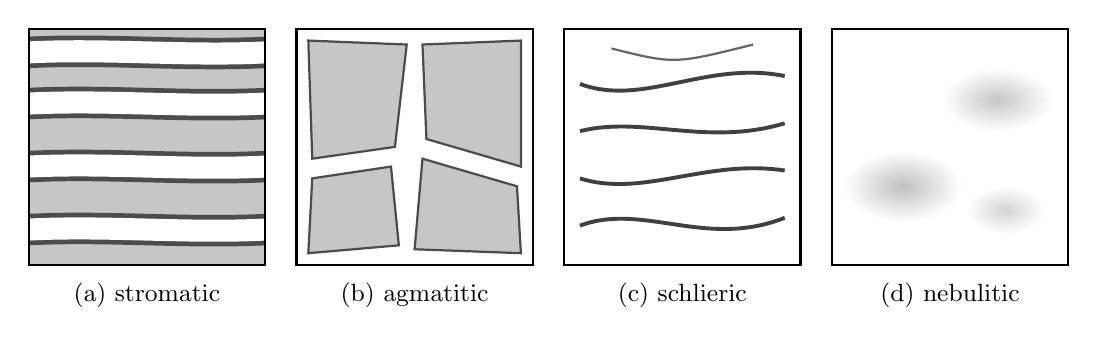
\begin{tikzpicture}[x=1cm, y=1cm]
% (a) stromatic
\begin{scope}
\fill[gray!45] (0,0) rectangle (3,3);
\foreach \y in {0.45, 1.25, 2.05, 2.7} {
  \fill[black!70] (0,\y-0.2) .. controls (1,\y-0.15) and (2,\y-0.25) .. (3,\y-0.2)
    -- (3,\y+0.2) .. controls (2,\y+0.15) and (1,\y+0.25) .. (0,\y+0.2) -- cycle;
  \fill[white] (0,\y-0.14) .. controls (1,\y-0.09) and (2,\y-0.19) .. (3,\y-0.14)
    -- (3,\y+0.14) .. controls (2,\y+0.09) and (1,\y+0.19) .. (0,\y+0.14) -- cycle;
}
\draw[thick] (0,0) rectangle (3,3);
\node[font=\small, anchor=north] at (1.5,-0.1) {(a) stromatic};
\end{scope}
% (b) agmatitic
\begin{scope}[xshift=3.4cm]
\fill[white] (0,0) rectangle (3,3);
\fill[gray!45, draw=black!70, thick] (0.15,0.15) -- (1.3,0.25) -- (1.2,1.25) -- (0.2,1.1) -- cycle;
\fill[gray!45, draw=black!70, thick] (1.5,0.2) -- (2.85,0.15) -- (2.8,1.0) -- (1.6,1.35) -- cycle;
\fill[gray!45, draw=black!70, thick] (0.2,1.35) -- (1.25,1.5) -- (1.4,2.8) -- (0.15,2.85) -- cycle;
\fill[gray!45, draw=black!70, thick] (1.65,1.6) -- (2.85,1.25) -- (2.85,2.85) -- (1.6,2.8) -- cycle;
\draw[thick] (0,0) rectangle (3,3);
\node[font=\small, anchor=north] at (1.5,-0.1) {(b) agmatitic};
\end{scope}
% (c) schlieric
\begin{scope}[xshift=6.8cm]
\fill[white] (0,0) rectangle (3,3);
\foreach \y/\a in {0.5/0.3, 1.1/-0.25, 1.7/0.2, 2.3/-0.3} {
  \draw[black!75, line width=1.4pt] (0.2,\y) .. controls (1,\y+\a) and (1.8,\y-\a) .. (2.8,\y+0.1);
}
\draw[black!60, line width=0.8pt] (0.6,2.75) .. controls (1.4,2.55) .. (2.4,2.8);
\draw[thick] (0,0) rectangle (3,3);
\node[font=\small, anchor=north] at (1.5,-0.1) {(c) schlieric};
\end{scope}
% (d) nebulitic
\begin{scope}[xshift=10.2cm]
\fill[white] (0,0) rectangle (3,3);
\shade[inner color=gray!50, outer color=white] (0.9,1.0) ellipse (0.75 and 0.45);
\shade[inner color=gray!45, outer color=white] (2.1,2.1) ellipse (0.7 and 0.4);
\shade[inner color=gray!35, outer color=white] (2.2,0.7) ellipse (0.5 and 0.3);
\draw[thick] (0,0) rectangle (3,3);
\node[font=\small, anchor=north] at (1.5,-0.1) {(d) nebulitic};
\end{scope}
\end{tikzpicture}
\par\smallskip{\small Four structures of \omterm{def:b2:crustal-melting:migmatite}{migmatites}, schematic (outcrop faces about a metre
across). White: \omterm{def:b2:crustal-melting:migmatite}{leucosome}; black: \omterm{def:b2:crustal-melting:migmatite}{melanosome}; grey: mesosome. (a) Stromatic: layers of
\omterm{def:b2:crustal-melting:migmatite}{leucosome}, each with a dark selvedge, parallel to the foliation, typical of \omterm{def:b2:crustal-melting:migmatite}{metatexites}.
(b) Agmatitic: a network of \omterm{def:b2:crustal-melting:migmatite}{leucosome} veins around angular blocks, giving a brecciated
look. (c) Schlieric: streaks of dark minerals within the \omterm{def:b2:crustal-melting:migmatite}{leucosome}. (d) Nebulitic: diffuse
ghosts of the earlier rock in an igneous-looking host; (c) and (d) are typical of
\omterm{def:b2:crustal-melting:migmatite}{diatexites}.}
\end{omfigure}
% ledger: bgs99:migmatite, scmr:migmatite

\begin{omfigure}
\centering
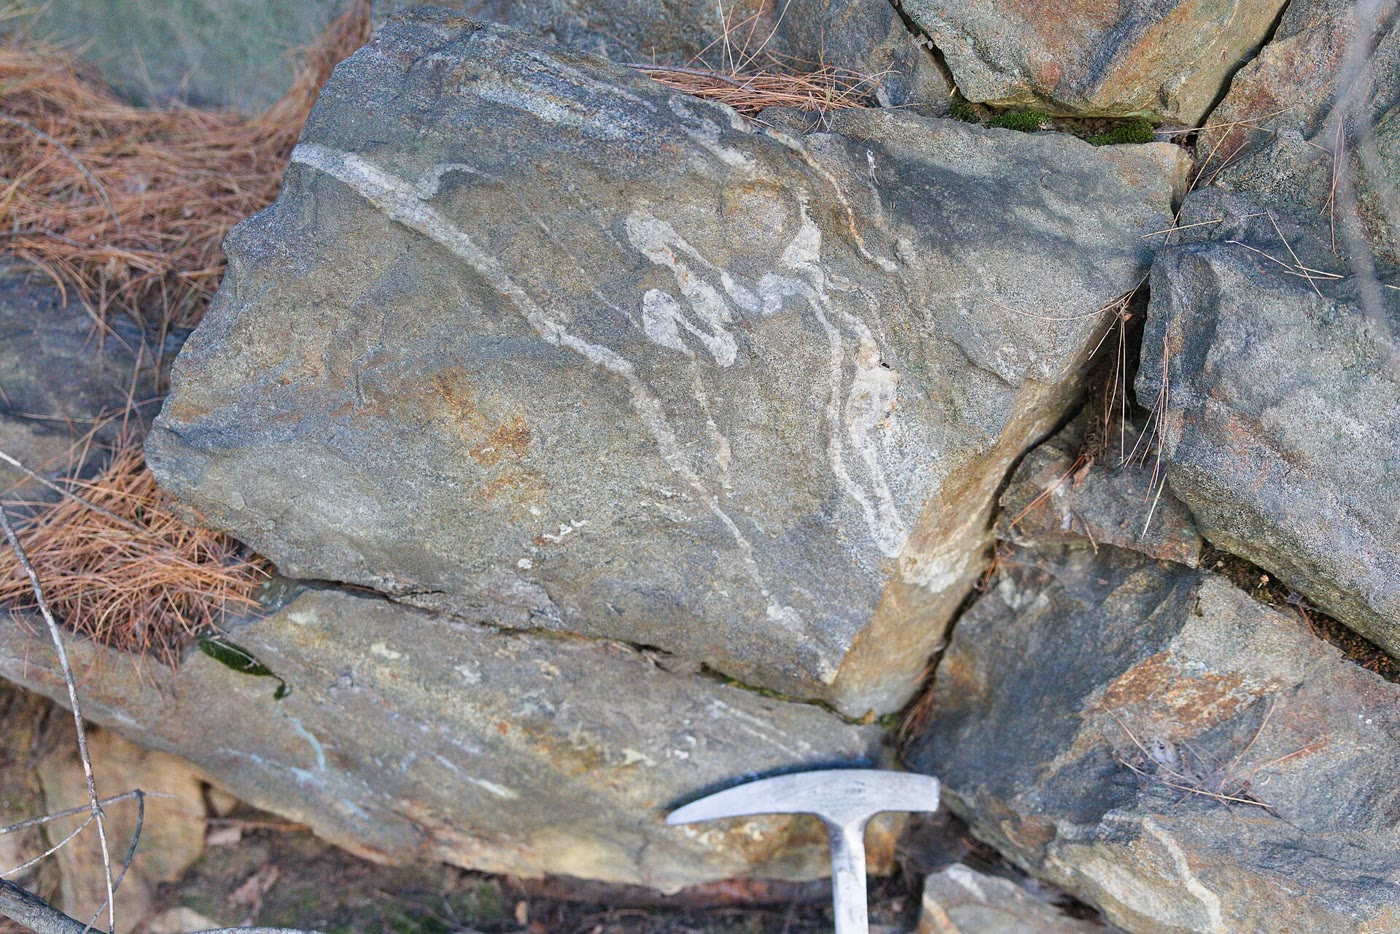
\includegraphics[width=0.62\linewidth]{images/book4/b2-12-migmatite.jpg}
\par\smallskip{\small A \omterm{def:b2:crustal-melting:migmatite}{migmatite} in Nashua, New Hampshire: light \omterm{def:b2:crustal-melting:migmatite}{leucosome} veins, folded
with the grey gneiss that holds them. The geologist's hammer gives the scale. Photograph Kevin M. Gill, CC BY 4.0.}
\end{omfigure}

\section{From migmatite to pluton}\label{sec:b2:crustal-melting:segregation}

At the grain scale, the first melt lies along the grain boundaries and in small pools,
mostly parallel to the foliation. Small as it is, it changes the rock: in experiments on
partially melted granite, the strength of the aggregate falls steeply between the solidus
and a \omterm{def:b2:mantle-melting:fraction}{melt fraction} of \num{0.07}, as the melt-bearing grain boundaries connect, and falls
again, by about four orders of magnitude but from an already low value, when the crystal
framework breaks down at higher \omterm{def:b2:mantle-melting:fraction}{melt fractions}. Partially molten crust is therefore weak,
and deformation gathers there as soon as melting starts. Deformation in turn drives the
melt: it drains from the matrix along linked grain boundaries into \omterm{def:b2:crustal-melting:migmatite}{leucosomes} parallel to
the foliation, then out of the melting layer through \omterm{def:b2:crustal-melting:migmatite}{leucosomes} that cut across it, and
these join into the \omterm{def:b2:magma-emplacement:bodies}{dykes} of \cref{ch:b2:magma-emplacement}. The figure below sums up the
path from the source to the \omterm{def:b2:magma-emplacement:bodies}{pluton}.
% ledger: sawyer01:segregation, rh05:connectivity

\begin{omfigure}
\centering
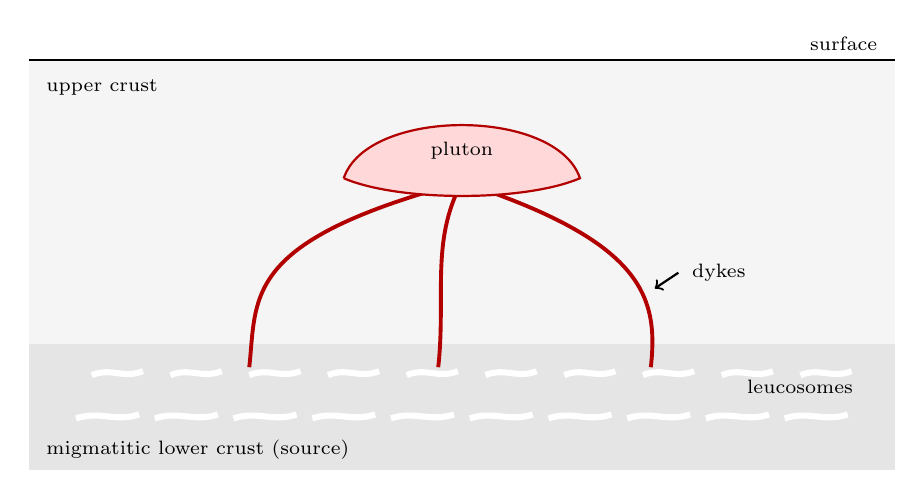
\begin{tikzpicture}[x=1cm, y=1cm]
\fill[gray!20] (0,0) rectangle (11,1.6);
\fill[gray!8] (0,1.6) rectangle (11,5.2);
\node[font=\scriptsize, anchor=west] at (0.1,0.25) {migmatitic lower crust (source)};
\foreach \x in {0.6,1.6,2.6,3.6,4.6,5.6,6.6,7.6,8.6,9.6} {
  \draw[white, line width=2.2pt] (\x,0.65) .. controls (\x+0.3,0.75) and (\x+0.5,0.6) .. (\x+0.8,0.7);
  \draw[white, line width=2.2pt] (\x+0.2,1.2) .. controls (\x+0.45,1.3) and (\x+0.6,1.15) .. (\x+0.85,1.25);
}
\foreach \x in {2.8, 5.2, 7.9} {
  \draw[red!70!black, line width=1.4pt] (\x,1.3) .. controls (\x+0.1,2.2) and (\x-0.1,2.9) .. (5.5,3.65);
}
\fill[pink!60, draw=red!70!black, thick] (4.0,3.7) .. controls (4.3,4.6) and (6.7,4.6) .. (7.0,3.7)
  .. controls (6.3,3.4) and (4.7,3.4) .. (4.0,3.7);
\node[font=\scriptsize] at (5.5,4.05) {pluton};
\node[font=\scriptsize, anchor=west] at (8.3,2.5) {dykes};
\draw[->, thick] (8.25,2.5) -- (7.95,2.3);
\node[font=\scriptsize, anchor=west] at (0.1,4.85) {upper crust};
\draw[thick] (0,5.2) -- (11,5.2);
\node[font=\scriptsize, anchor=south east] at (10.9,5.2) {surface};
\node[font=\scriptsize, align=left, anchor=west] at (9.0,1.05) {leucosomes};
\end{tikzpicture}
\par\smallskip{\small From \omterm{def:b2:crustal-melting:migmatite}{migmatite} to \omterm{def:b2:magma-emplacement:bodies}{pluton}, schematic and not to scale: \omterm{def:b2:crustal-melting:migmatite}{leucosomes}
(white) in the partially molten source join into \omterm{def:b2:magma-emplacement:bodies}{dykes} (red) that feed a \omterm{def:b2:magma-emplacement:bodies}{pluton} higher in
the crust.}
\end{omfigure}

How long does the crust stay molten? In the Himalaya, widespread \omterm{def:b2:crustal-melting:anatexis}{anatexis} began some
30 million years after the collision of India with Asia, and the zircon and monazite of the
anatectic rocks give ages from about 25 to 15 million years ago; a single sample may cover
most of this span. The melting of the Himalayan crust was not an event but a state that
lasted about ten million years.
% ledger: weinberg16:himalaya

\section{Granite types}\label{sec:b2:crustal-melting:types}

A granite remembers its source in its chemistry, first of all in how much aluminium it
has compared with what its feldspars can take.

\begin{definition}[Aluminium saturation index]\label{def:b2:crustal-melting:asi}
The \emph{aluminium saturation index}\index{aluminium saturation index} of a rock is the
molar ratio
\[\mathrm{A/CNK} = \frac{n(\ce{Al2O3})}{n(\ce{CaO}) + n(\ce{Na2O}) + n(\ce{K2O})},\]
and its companion is $\mathrm{A/NK} = n(\ce{Al2O3})/[n(\ce{Na2O}) + n(\ce{K2O})]$. A rock
is \emph{peraluminous}\index{peraluminous} if $\mathrm{A/CNK} > 1$,
\emph{metaluminous}\index{metaluminous} if $\mathrm{A/CNK} < 1 < \mathrm{A/NK}$, and
\emph{peralkaline}\index{peralkaline} if $\mathrm{A/NK} < 1$.
\end{definition}
% ledger: moyen17:aluminosity, frost01:asi

\begin{proposition}[What the index measures]\label{prop:b2:crustal-melting:feldspar}
A rock whose calcium, sodium and potassium are all in feldspars, and whose aluminium is
all in feldspars, has $\mathrm{A/CNK} = 1$. Hence a \omterm{def:b2:crustal-melting:asi}{peraluminous} rock has aluminium left
over after its feldspars, held in aluminous minerals (muscovite, garnet, cordierite,
aluminosilicate); a \omterm{def:b2:crustal-melting:asi}{metaluminous} rock has calcium left over, held in calcium silicates
(hornblende, clinopyroxene, titanite); and a \omterm{def:b2:crustal-melting:asi}{peralkaline} rock has sodium and potassium
left over, held in minerals without enough aluminium for feldspar (sodic pyroxene and
sodic amphibole).
\end{proposition}

\begin{proof}
In oxide form, K-feldspar is \ce{K2O.Al2O3.6SiO2}, albite \ce{Na2O.Al2O3.6SiO2} and
anorthite \ce{CaO.Al2O3.2SiO2}: each formula has exactly one \ce{Al2O3} for one
\ce{K2O}, \ce{Na2O} or \ce{CaO}. Any mixture of the three therefore has $n(\ce{Al2O3}) =
n(\ce{CaO}) + n(\ce{Na2O}) + n(\ce{K2O})$, that is $\mathrm{A/CNK} = 1$. If
$\mathrm{A/CNK} > 1$, the aluminium exceeds what the alkalis and calcium can bind into
feldspar, and the excess must sit in other minerals. If $\mathrm{A/CNK} < 1$ but
$\mathrm{A/NK} > 1$, there is enough aluminium for all the sodium and potassium as
feldspar but not for all the calcium, which goes into minerals that need less aluminium
per calcium than anorthite. If $\mathrm{A/NK} < 1$, even the alkalis cannot all be in
feldspar.
\end{proof}

Moyen and colleagues found aluminosity the most useful indicator for telling granites
with different sources apart; Frost and colleagues use the same index, with a small
correction for phosphorus, as one of the three axes of their classification of granitic
rocks.
% ledger: moyen17:aluminosity, frost01:asi

\begin{omfigure}
\centering
\begin{tikzpicture}
\begin{axis}[omrecord, width=0.72\linewidth, height=7cm,
  xmin=0.4, xmax=1.5, ymin=0.4, ymax=3.5, xlabel={A/CNK (molar)}, ylabel={A/NK (molar)},
  tick label style={font=\scriptsize}, label style={font=\small}]
\addplot[fill=gray!15, draw=none] coordinates {(0.4,0.4) (1.5,1.5) (1.5,0.4) (0.4,0.4)};
\addplot[thick, black!70] coordinates {(1,0.4) (1,3.5)};
\addplot[thick, black!70] coordinates {(0.4,1) (1.5,1)};
\node[font=\scriptsize, anchor=north east] at (axis cs:1.48,3.45) {peraluminous};
\node[font=\scriptsize, anchor=west] at (axis cs:0.62,2.6) {metaluminous};
\node[font=\scriptsize, anchor=south west] at (axis cs:0.42,0.45) {peralkaline};
\addplot[only marks, mark=*, mark size=2pt, blue!70!black, nodes near coords,
  point meta=explicit symbolic, every node near coord/.style={font=\scriptsize, anchor=west}]
  coordinates {(0.539,3.196)[BHVO-2] (0.877,1.694)[AGV-2] (0.993,1.135)[SRM 278]};
\addplot[only marks, mark=square*, mark size=2pt, red!70!black]
  coordinates {(1.261,1.377) (0.809,0.844)};
\node[font=\scriptsize, red!70!black, anchor=south] at (axis cs:1.261,1.45) {S-type melt};
\node[font=\scriptsize, red!70!black, anchor=north] at (axis cs:0.809,0.79) {peralkaline granite};
\end{axis}
\end{tikzpicture}
\par\smallskip{\small Shand's diagram. Blue circles: three reference materials, a Hawaiian
basalt (BHVO-2), an andesite (AGV-2) and an obsidian of granitic composition (SRM 278),
computed from their published oxide contents. Red squares: two invented granites used in
this chapter. The grey triangle cannot be reached, since A/CNK never exceeds A/NK.}
\end{omfigure}
% ledger: usgs:bhvo2-major, usgs:agv2-major, nist278:majors

The chemistry follows the source. In 1974, Chappell and White noticed that, apart from the
most felsic rocks, the granites of the Lachlan Fold Belt fall into two distinct groups,
and interpreted them as melts of two kinds of source rock: older igneous rocks and sedimentary rocks. The hydrolysis of feldspars, seen in the Year 1
volume, carries sodium and calcium away in solution and keeps aluminium in clays: muds made
of these clays are rich in aluminium, and so are their melts.
% ledger: cw01:is-types

\begin{definition}[Granite typology]\label{def:b2:crustal-melting:types}
An \emph{I-type granite}\index{I-type granite} is a granite whose source was dominantly an
older igneous rock, an \emph{S-type granite}\index{S-type granite} one whose source was
dominantly a sedimentary (metasedimentary) rock, and an M-type granite one derived from
the mantle. An \emph{A-type granite}\index{A-type granite} is defined by its chemistry and
setting rather than its source: ferroan and potassic, strongly enriched in \omterm{def:b2:elements-in-the-earth:partition}{incompatible
elements}, and emplaced in stable intra-plate, back-arc or post-collisional settings.
\end{definition}
% ledger: johansson23:a-type, cw01:is-types

\omterm{def:b2:crustal-melting:types}{S-type granites} are \omterm{def:b2:crustal-melting:asi}{peraluminous}, with two micas or with cordierite; A-type granitoids
are mostly \omterm{def:b2:crustal-melting:asi}{metaluminous}, some \omterm{def:b2:crustal-melting:asi}{peraluminous}. A single analysis can mislead, though: every
granitoid suite ends near the composition of the granitic minimum, leucocratic and mildly
\omterm{def:b2:crustal-melting:asi}{peraluminous}, so a \omterm{def:b2:crustal-melting:asi}{peraluminous} sample is no proof that crust was melted. What tells
suites apart is the shape of their trend in Shand's diagram: an arc suite reaches the
minimum along a steep array from high A/NK and low A/CNK, a low-calcium S-type suite
along an array with A/NK close to A/CNK. No consensus has been reached on the source of
A-type \omterm{def:b2:magma-emplacement:magma}{magmas}: one model makes them from underplated basalt, evolved by crystallisation,
\omterm{def:b2:mantle-melting:melting}{partial melting} and assimilation of crust.
% ledger: moyen17:trends, frost01:asi, johansson23:a-type

\begin{definition}[Leucogranite]\label{def:b2:crustal-melting:leucogranite}
A \emph{leucogranite}\index{leucogranite} is a light-coloured granite, almost free of
dark minerals; the \omterm{def:b2:crustal-melting:asi}{peraluminous} leucogranites of collision belts carry muscovite, alone or
with biotite.
\end{definition}
% ledger: moyen17:aluminosity, pdh98:himalaya

The muscovite-bearing \omterm{def:b2:crustal-melting:asi}{peraluminous} \omterm{def:b2:crustal-melting:leucogranite}{leucogranites} of collision belts have compositions close
to the liquids of water-present or muscovite \omterm{def:b2:crustal-melting:reactions}{dehydration melting}, at temperatures near
\qty{700}{\celsius} where zircon and monazite of the source can survive and be carried
into the melt as xenocrysts; cordierite-bearing \omterm{def:b2:crustal-melting:asi}{peraluminous} granites come from the
hotter breakdown of biotite, at 800 to \qty{850}{\celsius}. The Himalayan \omterm{def:b2:crustal-melting:leucogranite}{leucogranites},
with their strong crustal isotopic signature, belong to this family
(\cref{ch:b2:himalaya-andes}).
% ledger: moyen17:aluminosity, weinberg16:himalaya

\begin{omfigure}
\centering
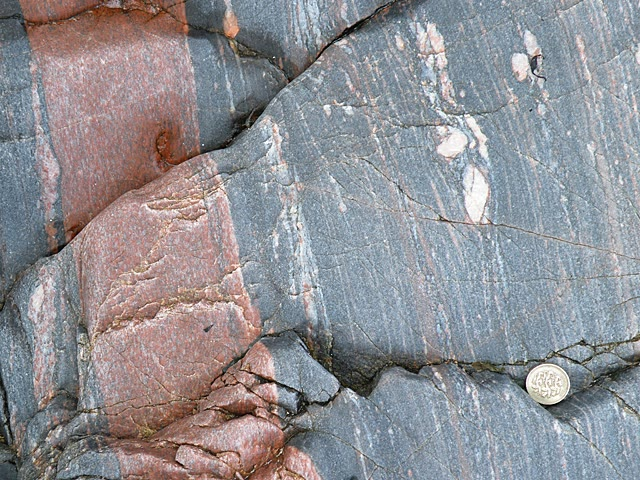
\includegraphics[width=0.5\linewidth]{images/book4/b2-12-leucogranite-vein.jpg}
\par\smallskip{\small A pink \omterm{def:b2:crustal-melting:leucogranite}{leucogranite} vein cutting a banded grey gneiss; the coin gives
the scale. Photograph Anne Burgess (Geograph), CC BY-SA 2.0.}
\end{omfigure}

\section{Granites and the growth of continents}\label{sec:b2:crustal-melting:time}

Two kinds of places make most granite. Above subduction zones, arc crust forms by the
differentiation of mafic melts from the mantle, and the heat available is only what these
melts bring. After a collision, the thickened crust is a very hot system: it melts on a
large scale, at low temperature where water or muscovite allows it and at higher
temperature by biotite breakdown, and these crust-derived granites recycle crust that
already existed. Mantle melts reach the crust there too, in amounts large enough, Moyen and
colleagues argue, to make late-orogenic belts important contributors to the growth of the
crust. Whether a granite adds to the continents or only reworks them is thus a question of
its source, which its isotopes answer (\cref{ch:b2:isotope-geochemistry}); the granites of
the early Earth, very different from these, are the subject of
\cref{ch:b2:precambrian-earth}.
% ledger: moyen17:settings

\section{Exercises}\label{sec:b2:crustal-melting:exercises}

Molar masses (\unit{\gram\per\mole}): \ce{Al2O3} 101.96, \ce{CaO} 56.08, \ce{Na2O} 61.98,
\ce{K2O} 94.20, \ce{H2O} 18.02; atomic masses: H 1.008, O 16.00, Na 22.99, Mg 24.31,
Al 26.98, Si 28.09, K 39.10, Ca 40.08. Take $g = \qty{9.81}{\metre\per\second\squared}$.

\begin{exercise}[$\star$]\label{exo:b2:crustal-melting:1}
The andesite reference material AGV-2 contains, in \unit{\gram} per \qty{100}{\gram},
\ce{Al2O3} 17.03, \ce{CaO} 5.15, \ce{Na2O} 4.204 and \ce{K2O} 2.898.
(a) Compute its A/CNK and A/NK. (b) Classify it, and name a mineral that should hold its
excess calcium.
\end{exercise}
% ledger: usgs:agv2-major

\begin{exercise}[$\star$]\label{exo:b2:crustal-melting:2}
Three granites contain, besides quartz and feldspars: (a) muscovite, biotite and garnet;
(b) hornblende, biotite and titanite; (c) aegirine, a sodium--iron pyroxene
\ce{NaFeSi2O6}, and a sodic amphibole. Classify each by its aluminium saturation, and say
which could be an \omterm{def:b2:crustal-melting:types}{S-type granite}.
\end{exercise}

\begin{exercise}[$\star$]\label{exo:b2:crustal-melting:3}
A crust of density \qty{2800}{\kilogram\per\cubic\metre} has a linear geotherm
$T = \qty{10}{\celsius} + (\qty{20}{\celsius\per\kilo\metre})\,z$. Between 2 and
\qty{10}{kbar}, approximate the wet granite solidus by the straight line through
(\qty{680}{\celsius}, \qty{2}{kbar}) and (\qty{620}{\celsius}, \qty{10}{kbar}). At what
depth, temperature and pressure does the geotherm meet it?
\end{exercise}
% ledger: sw81:wet-solidus

\begin{exercise}[$\star$]\label{exo:b2:crustal-melting:4}
A grey biotite gneiss carries centimetre-thick white layers of quartz and feldspar, parallel
to its foliation, each bordered by a thin black seam of biotite; between the layers the
gneiss looks ordinary. (a) Name the white layers, the black seams and the ordinary gneiss.
(b) Is the rock a \omterm{def:b2:crustal-melting:migmatite}{metatexite} or a \omterm{def:b2:crustal-melting:migmatite}{diatexite}, and what is its structure? (c) A few hundred
metres away, the layering has gone: a streaky, granite-like rock holds faint ghosts of
gneiss. What has changed?
\end{exercise}
% ledger: scmr:migmatite, bgs99:migmatite

\begin{exercise}[$\star\star$]\label{exo:b2:crustal-melting:5}
Take biotite as phlogopite, \ce{KMg3AlSi3O10(OH)2}. (a) Compute its molar mass and the
mass fraction of water it releases (its two hydroxyl groups give one \ce{H2O}).
(b) A gneiss with \qty{25}{\percent} biotite by mass melts by biotite \omterm{def:b2:crustal-melting:reactions}{dehydration melting}
into a melt holding \qty{4.0}{\percent} water. Using
\cref{prop:b2:crustal-melting:water}, find the \omterm{def:b2:mantle-melting:fraction}{melt fraction}, and compare it with the
fractions found in experiments on biotite \omterm{def:b2:crustal-melting:reactions}{dehydration melting}.
\end{exercise}
% ledger: bk99:migmatites

\begin{exercise}[$\star\star$]\label{exo:b2:crustal-melting:6}
A hundred grams of granite contain \qty{30}{\gram} of K-feldspar \ce{KAlSi3O8},
\qty{35}{\gram} of albite \ce{NaAlSi3O8}, \qty{5}{\gram} of anorthite \ce{CaAl2Si2O8},
\qty{25}{\gram} of quartz and \qty{5}{\gram} of muscovite \ce{KAl3Si3O10(OH)2}.
(a) Compute the molar masses of the four aluminous minerals. (b) Compute the amounts of
\ce{Al2O3}, \ce{CaO}, \ce{Na2O} and \ce{K2O} in the rock, and its A/CNK. (c) Which
mineral makes the rock \omterm{def:b2:crustal-melting:asi}{peraluminous}?
\end{exercise}

\begin{exercise}[$\star\star$]\label{exo:b2:crustal-melting:7}
A basaltic \omterm{def:b2:magma-emplacement:bodies}{sill} intruded at \qty{1200}{\celsius} crystallises completely and cools to
\qty{850}{\celsius}, releasing a latent heat of \qty{900}{\mega\joule\per\cubic\metre}.
The crust around it, at \qty{650}{\celsius}, is heated to \qty{850}{\celsius} and
\qty{20}{\percent} of it melts, with the same latent heat per unit volume of melt. Both
rocks have a heat capacity of \qty{2.5}{\mega\joule\per\cubic\metre\per\kelvin}. Using
\cref{prop:b2:crustal-melting:heat}, how many cubic metres of crust can one cubic metre
of basalt treat this way? What does the result ignore?
\end{exercise}
% ledger: delaney86b4:properties

\begin{exercise}[$\star\star$]\label{exo:b2:crustal-melting:8}
The obsidian reference material SRM 278 is certified at \ce{Al2O3}
$14.15 \pm 0.15$, \ce{CaO} 0.983, \ce{Na2O} 4.84 and \ce{K2O} 4.16 (\unit{\percent} by
mass). (a) Compute its A/CNK and A/NK and classify it. (b) Recompute A/CNK with the two
ends of the \ce{Al2O3} uncertainty. Is the classification robust?
\end{exercise}
% ledger: nist278:majors

\begin{exercise}[$\star\star$]\label{exo:b2:crustal-melting:9}
At \qty{800}{\celsius}, a haplogranite melt saturated in water holds \qty{7.45}{\percent}
water at \qty{3}{kbar}, 8.94 at \qty{4}{kbar}, 9.97 at \qty{5}{kbar} and 13.82 at
\qty{8}{kbar}. (a) Fit a straight line to these four points by least squares and compare
its slope with the \qty{1.27}{\percent} per kilobar quoted by the experimenters.
(b) Predict the saturation content at \qty{6}{kbar}. (c) What is the least mass of melt
that can carry \qty{10}{\gram} of water at \qty{6}{kbar}? (d) Why should the line not be
used at \qty{15}{kbar}?
\end{exercise}
% ledger: holtz95:solubility

\begin{exercise}[$\star\star\star$]\label{exo:b2:crustal-melting:10}
Approximate the dehydration-melting solidus of a muscovite schist by the straight line
through (\qty{750}{\celsius}, \qty{6}{kbar}) and (\qty{800}{\celsius}, \qty{10}{kbar}),
the ends of the experimental brackets. A schist at \qty{770}{\celsius} rises from
\qty{10}{kbar} without gaining or losing heat. (a) At what pressure does it reach the
solidus? (b) Beyond, its temperature follows the solidus down, the heat for melting coming
from its own cooling. With a heat capacity of \qty{2.5}{\mega\joule\per\cubic\metre\per\kelvin}
and a latent heat of \qty{900}{\mega\joule\per\cubic\metre}, what volume fraction of melt
has formed when it reaches \qty{6}{kbar}? (c) Compare with the conditions proposed for the
Himalayan \omterm{def:b2:crustal-melting:leucogranite}{leucogranites}.
\end{exercise}
% ledger: pdh98:himalaya, delaney86b4:properties

\begin{exercise}[$\star\star\star$]\label{exo:b2:crustal-melting:11}
Heat diffuses over a distance $\ell$ in a time of order $\ell^2/\kappa$. With
$\kappa = \qty{1e-6}{\square\metre\per\second}$, estimate the time for the heat of a
\qty{2}{km}-thick \omterm{def:b2:magma-emplacement:bodies}{sill}, and of a \qty{10}{km}-thick underplated layer, to spread over its
own thickness. Compare with the ten million years of Himalayan \omterm{def:b2:crustal-melting:anatexis}{anatexis}: can one
underplating event explain it?
\end{exercise}
% ledger: delaney86b4:properties, weinberg16:himalaya

\begin{exercise}[$\star\star\star$]\label{exo:b2:crustal-melting:12}
A stromatic \omterm{def:b2:crustal-melting:migmatite}{migmatite} is analysed: \omterm{def:b2:crustal-melting:migmatite}{leucosome} \ce{K2O} \qty{5.0}{\percent}, \ce{MgO}
\qty{0.20}{\percent}; \omterm{def:b2:crustal-melting:migmatite}{melanosome} \ce{K2O} \qty{2.0}{\percent}, \ce{MgO}
\qty{4.0}{\percent}; mesosome, taken as the unmelted parent, \ce{K2O}
\qty{2.75}{\percent}, \ce{MgO} \qty{3.05}{\percent} (all by mass). (a) If the
neosome formed from the parent without gain or loss, what mass fraction of it is
\omterm{def:b2:crustal-melting:migmatite}{leucosome}? (b) Check the answer with \ce{MgO}. (c) On the outcrop the \omterm{def:b2:crustal-melting:migmatite}{leucosome} makes only
\qty{10}{\percent} of the neosome by mass. How many grams of melt left per
\qty{100}{\gram} of parent rock?
\end{exercise}

\begin{problem}[{Weekend problem --- a pluton from melted mica}]\label{pb:b2:crustal-melting:1}
A schist made of \qty{20}{\percent} muscovite, \qty{15}{\percent} biotite,
\qty{30}{\percent} quartz, \qty{30}{\percent} plagioclase and \qty{5}{\percent} other
minerals (by mass; an invented rock) lies at the base of a crust doubled by stacking, the
situation modelled in \cref{ch:b2:pt-paths}. It may melt and feed a granite \omterm{def:b2:magma-emplacement:bodies}{pluton}. Data:
the atomic and molar masses at the head of the exercises; the wet granite solidus passes
through (\qty{680}{\celsius}, \qty{2}{kbar}), (\qty{620}{\celsius}, \qty{10}{kbar}),
(\qty{605}{\celsius}, \qty{15.3}{kbar}) and (\qty{670}{\celsius}, \qty{27}{kbar}); the
water saturation content of a granitic melt at \qty{800}{\celsius} is \qty{9.97}{\percent} at
\qty{5}{kbar} and \qty{13.82}{\percent} at \qty{8}{kbar}. The model base of the thickened crust follows:

\smallskip
\begin{center}\small
\begin{tabular}{l|ccccccccccc}
$t$ (\unit{Myr}) & 0 & 10 & 20 & 30 & 40 & 50 & 60 & 70 & 80 & 90 & 100\\ \hline
$T$ (\unit{\celsius}) & 595 & 656 & 734 & 795 & 845 & 885 & 909 & 914 & 900 & 867 & 814\\
$P$ (\unit{kbar}) & 19.2 & 19.2 & 19.2 & 19.2 & 17.9 & 16.5 & 15.1 & 13.7 & 12.4 & 11.0 & 9.6
\end{tabular}
\end{center}
\smallskip

\noindent\textbf{Part I --- Water from mica.}
\begin{enumerate}
\item Compute the molar mass of muscovite \ce{KAl3Si3O10(OH)2}.
\item Its two hydroxyl groups give one \ce{H2O}. What mass fraction of the mineral is
released as water?
\item How much water does the muscovite of one kilogram of schist release?
\item Interpolating linearly, what is the saturation water content of the melt at
\qty{7}{kbar}? What is then the least \omterm{def:b2:mantle-melting:fraction}{melt fraction} the muscovite water can make?
\item The melt of \omterm{def:b2:crustal-melting:reactions}{dehydration melting} is far from saturated; take its water content as
\qty{6.0}{\percent}. What \omterm{def:b2:mantle-melting:fraction}{melt fraction} does the muscovite make?
\item In experiments on a two-mica \omterm{def:b2:metamorphic-facies:protoliths}{metapelite} at \qty{10}{kbar}, the muscovite reaction
gave only 1 to \qty{2}{\percent} of melt. Name two reasons why a real rock may make less
melt than your answer to question~5.
\end{enumerate}

\noindent\textbf{Part II --- Heating the source.}
\begin{enumerate}[resume]
\item In \cref{ch:b2:pt-paths}, the rock left at mid-crust peaks at \qty{593}{\celsius}
and \qty{7.8}{kbar}. What is the wet solidus at \qty{7.8}{kbar}? Can that rock melt, even
with free water?
\item Interpolating between 15.3 and \qty{27}{kbar}, find the wet solidus at the pressure
of the base just after stacking. Is the base above it at $t = 0$? At $t = \qty{10}{Myr}$?
\item What limits the melting of the base at $t = \qty{10}{Myr}$, and why does it stop
soon?
\item When does the base pass \qty{800}{\celsius}, the upper end of the muscovite
bracket?
\item The amphibole bracket spans 875 to \qty{925}{\celsius} at 10 to \qty{12.5}{kbar}.
When does the base enter this pressure range, and at what temperature?
\item When does the base reach \qty{10}{kbar}, the top of the pressure range of the
muscovite experiments, and how hot is it then? Which hydrous minerals of the schist can
still exist?
\end{enumerate}

\noindent\textbf{Part III --- What melt?}
The melt, once crystallised, gives a \omterm{def:b2:crustal-melting:leucogranite}{leucogranite} (invented analysis) with, in
\unit{\percent} by mass, \ce{Al2O3} 15.0, \ce{CaO} 0.55, \ce{Na2O} 3.4 and \ce{K2O} 4.9.
\begin{enumerate}[resume]
\item Compute the amounts of the four oxides in \qty{100}{\gram} of the rock.
\item Compute its A/CNK.
\item Compute its A/NK and classify the \omterm{def:b2:crustal-melting:leucogranite}{leucogranite}.
\item Is it an I-type or an \omterm{def:b2:crustal-melting:types}{S-type granite}? Name two minerals that should hold its excess
aluminium.
\item How many moles of \ce{Al2O3} per \qty{100}{\gram} are left over after the
feldspars? If all of it went into muscovite, which holds one more \ce{Al2O3} per formula
unit than K-feldspar, how many grams of muscovite would \qty{100}{\gram} of granite
contain?
\item The obsidian SRM 278 has A/CNK $= 0.993$. Could the \omterm{def:b2:crustal-melting:leucogranite}{leucogranite} and the obsidian
come from the same kind of source?
\end{enumerate}

\noindent\textbf{Part IV --- How much crust?}
An invented \omterm{def:b2:magma-emplacement:bodies}{pluton} of this \omterm{def:b2:crustal-melting:leucogranite}{leucogranite} has a volume of \qty{1000}{\cubic\kilo\metre}.
Take \qty{2650}{\kilogram\per\cubic\metre} for the granite and
\qty{2800}{\kilogram\per\cubic\metre} for the schist; suppose \qty{70}{\percent} of the
melt leaves its source and all the melt's water escapes when it crystallises.
\begin{enumerate}[resume]
\item What is the mass of the \omterm{def:b2:magma-emplacement:bodies}{pluton}?
\item What mass of melt (with its \qty{6.0}{\percent} water) did it take?
\item Using the \omterm{def:b2:mantle-melting:fraction}{melt fraction} of question~5, what mass of schist had to melt?
\item What volume of schist is that?
\item If the source was a layer \qty{5}{km} thick, over what area did it melt?
\item With the least \omterm{def:b2:mantle-melting:fraction}{melt fraction} of question~4 instead, how much larger would the
source be? Give the volume of source crust melted to make the \omterm{def:b2:magma-emplacement:bodies}{pluton}, in
\unit{\cubic\kilo\metre}, from question~22.
\end{enumerate}
\end{problem}
